\chapter{Einleitung}

Die prozedurale Generierung von 3D-Modellen stellt einen wichtigen Bereich der Computergrafik dar. Im folgenden Kapitel werden bisherige Arbeiten zur Generierung von Baumstrukturen, die in dieser Arbeit umgesetzten Verfahren sowie das zur Implementierung verwendete Framework vorgestellt. 

\section{Prozedurale Generierung von Baumstrukturen}

Die Gestaltung von 3D-Modellen für die Computergrafik erfordert den sicheren Umgang mit 3D-Modellierungssoftware, künstlerisches Geschick und einen hohen Zeitaufwand. Im Bereich der Filmindustrie werden 3D-Modelle eingesetzt, um reale Schauspieler mit virtuellen Umgebungen verschmelzen zu lassen oder Filme allein durch Computersimulation zu erstellen. \cite[S.5]{Deussen:05} In Computerspielen werden Modelle verwendet, um beispielsweise virtuelle Charaktere und die sie umgebenden Landschaften darzustellen. Um diese Aufgaben zu erfüllen besteht ein Großteil der Entwicklungsteams aus 3D-Künstlern, welche für die Erstellung der 3D-Modelle verantwortlich sind. \cite[S.3]{PCGiG:16}

Die Prozedurale Generierung von Modellen ist ein Ansatz für eine schnellere Erfüllung dieser Aufgaben bei geringerem Aufwand und äquivalenter Qualität. Dabei werden 3D-Modelle durch computergenerierte Daten, auf Basis von Algorithmen und mit eingeschränktem Eingriff durch einen Benutzer, erstellt. \cite[S.1]{PCGiG:16} 

\begin{figure} [htbp]
	\centering
	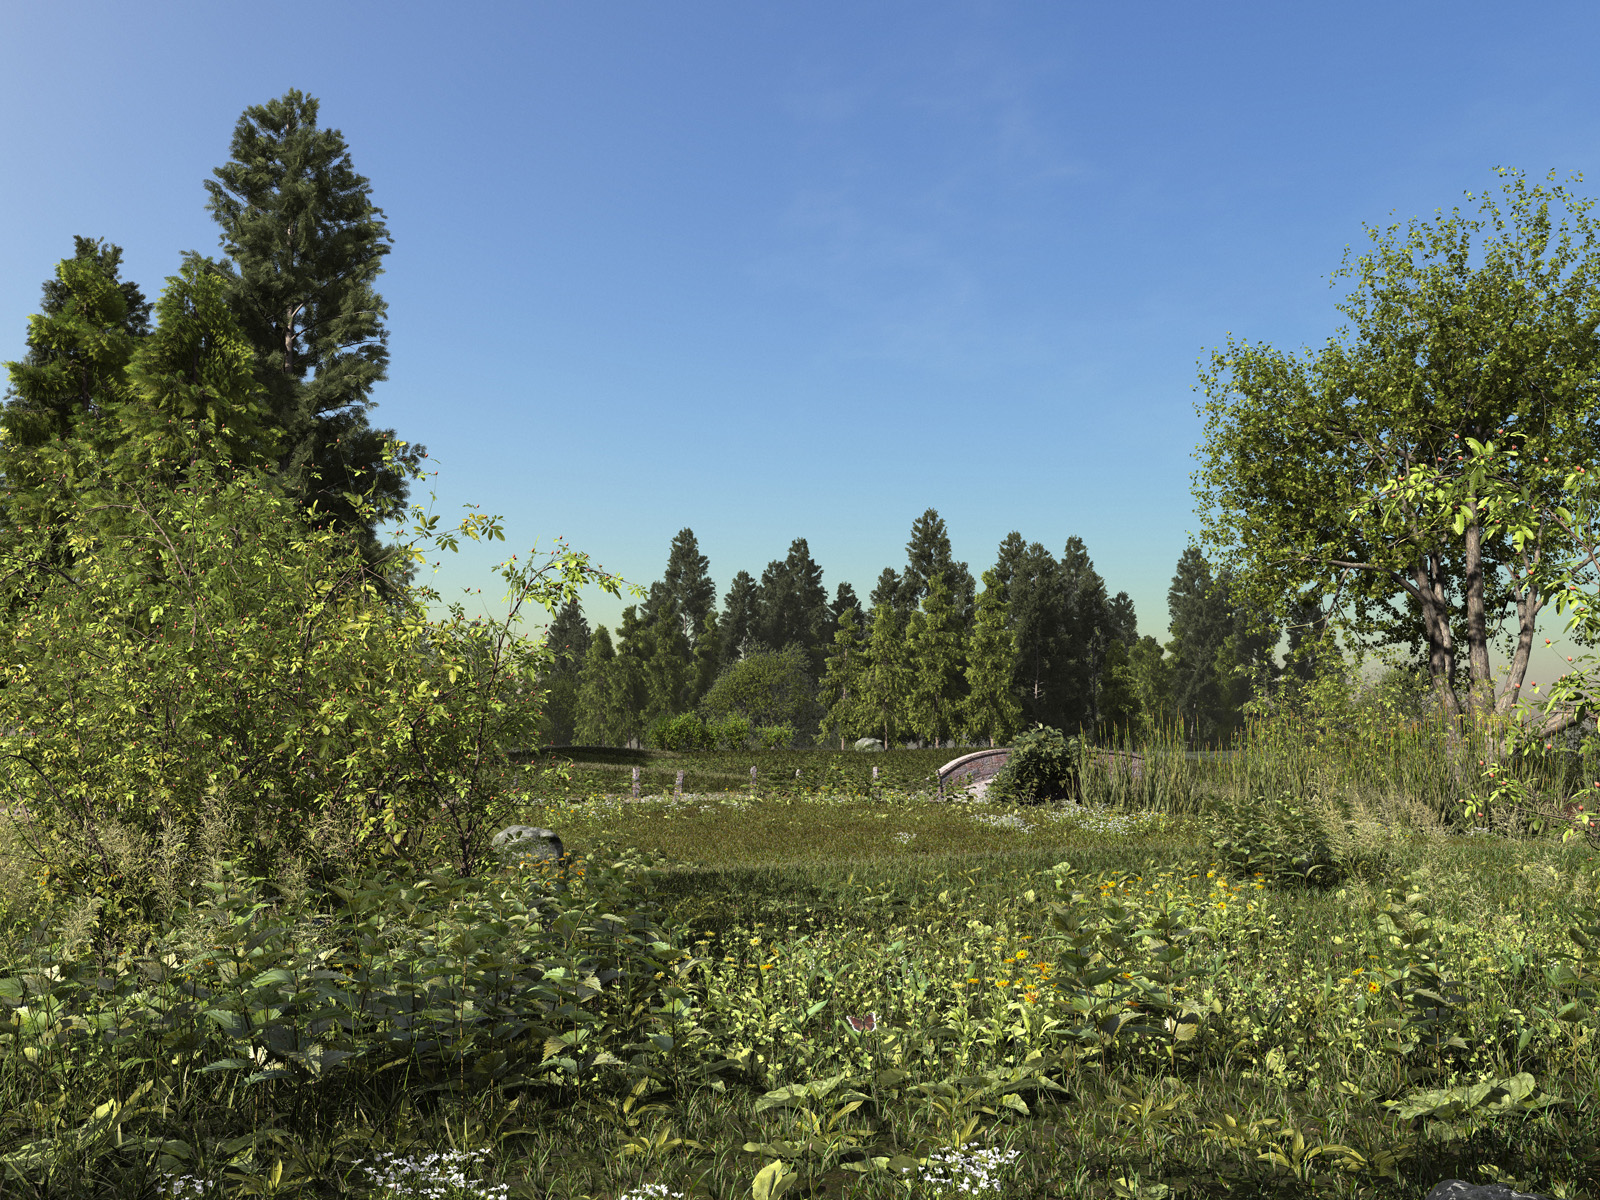
\includegraphics[width=.7\textwidth]{images/greenXfrog_JanWalterSchliep.jpg}
	\caption{\glqq Green\grqq{} von Jan Walter Schliep, modelliert mithilfe der prozeduralen 3D-Modellierungssoftware für Vegetation, \glqq Xfrog\grqq. \cite{GreenOne:16}}
	\label{fig:greenXfrog_JanWalterSchliep}
\end{figure}

Die Generierung von Pflanzenmodellen stellt einen großen Bereich der prozeduralen Modellgenerierung dar, da es nur in Ausnahmefällen möglich ist Szenen von Außenbereichen zu erzeugen ohne Vegetation darzustellen. Die Komplexität dieser Thematik wird bereits bei der Betrachtung einzelner Pflanzen deutlich und erstreckt sich von der Modellierung eines einzelnen Blattes über die Positionierung der Blätter auf einer Pflanze bis hin zur Verteilung dieser Vegetation in einer Landschaft. \cite[S.3]{Deussen:05} Eine simple Wiederverwendung von Modellen wird schnell bemerkt und führt zu einem unnatürlichen Eindruck bei Beobachtern -- die manuelle Gestaltung von 3D-Modellen ist somit selten praktikabel. \cite[S.73]{PCGiG:16}

Bäume stellen auffällige Landschaftsmerkmale dar und sind somit ein wichtiger Bestandteil einer realistischen Umgebungsgestaltung. Im Rahmen dieser Arbeit werden daher zwei unterschiedliche Verfahren für die prozedurale Generierung der Aststrukturen von Bäumen sowie die jeweiligen Implementierungen in einer -- insbesondere für die Verwendung in digitalen Spielen geeigneten -- Echtzeitanwendung vorgestellt. 

\section{Bisherige Arbeiten}

Die Entwicklung von Programmen für die 3D-Modellgenerierung von Baumstrukturen begann mit den Arbeiten von Honda und Fisher sowie den Erweiterungen dieser durch Aono und Kunii. Sie verwendeten einige simple Regeln, die mithilfe von Parametern angepasst werden konnten, um realistisch wirkende Baumstrukturen zu erschaffen. \cite[S.46f]{Deussen:05} \cite[S.1]{SpaceColonizationAlgorithm:07} 

Die bereits zuvor von Aristid Lindenmayer entwickelte Erweiterung von kontextfreien Grammatiken -- Lindenmayer-Systeme -- für die Beschreibung zellulärer Vorgänge und das Verzweigungsverhalten von Pflanzen wurden später von Prusinkiewicz und Lindenmayer zusätzlich erweitert, um die Generierung ähnlicher Baumstrukturen mithilfe dieser Systeme zu ermöglichen. \cite[S.43, 48]{Deussen:05} 

Die von P. Oppenheimer und J. Bloomenthal entwickelten Verfahren basieren auf der rekursiven Generierung von Baumstrukturen. Oppenheimers Vorgehen war inspiriert durch die fraktale Natur von Pflanzen und konzentriert auf die schnelle grafische Repräsentation der Modelle, während Bloomenthal die natürliche Darstellung von Verzweigungen beabsichtigte. \cite[S.49-52]{Deussen:05} 

Weiterhin trugen Reeves und Blau, Weber und Penn, Lintermann und Deussen sowie Prusinkiewicz u.a zur Verbesserung und Erweiterung von rekursiven Prozeduren zur Generierung von realistischen Baumstrukturen bei. \cite[S.1]{SpaceColonizationAlgorithm:07}

Ein Ansatz, der sich vom rekursiven Vorgehen unterscheidet, wurde von Rodkaew u.a. entwickelt und basiert auf der Verteilung von Partikeln in Form einer Baumkrone um daraufhin die Aststruktur iterativ von außen bis zur Wurzel aufzubauen. \cite[S.2]{SpaceColonizationAlgorithm:07} Diesem Ansatz ähnelt das Vorgehen von Runions u.a., welches die Erweiterung eines zweidimensionalen Verfahrens zur Generierung von Blattvenen in den dreidimensionalen Raum darstellt und als Space Colonization Algorithmus (engl. für Raum-Kolonisierungs-Algorithmus) bezeichnet wird. Im Gegensatz zu Rodkaew u.a. wurde jedoch der iterative Aufbau ausgehend von der Wurzel und in Abhängigkeit des verfügbaren Raums zum Wachsen vorgeschlagen. \cite[S.2]{SpaceColonizationAlgorithm:07}


\section{Ansatz}

Im Rahmen dieser Arbeit wurden zwei verschiedene Verfahren implementiert: Die von Aristid Lindenmayer entwickelten Lindenmayer-Systeme sowie der von Runions u.a. entwickelte Space Colonization Algorithmus. 

Lindenmayer-Systeme arbeiten mithilfe einer vorgegebenen Menge von Regeln, um bestimmte Teile einer Zeichenkette durch andere Zeichen zu ersetzen. Diese Regeln verlängern die ursprüngliche Zeichenkette und ermöglichen somit die Generierung von komplexen Zeichenabfolgen. \cite[S.2]{ABOP:04} Um aus den Resultaten Modelldaten zu extrahieren wird die von Prusinkiewicz und Lindenmayer vorgeschlagene Interpretation von Zeichenketten verwendet. \cite[S.6]{ABOP:04}

Der Space Colonization Algorithmus nutzt die biologisch motivierte Simulation von Konkurrenz um Platz zwischen sich entwickelnden Zweigen. Es wird ein bestimmter Wachstumsbereich vorgegeben, in dem Zweige in jeder Iteration des Algorithmus wachsen. \cite[S.5]{SpaceColonizationAlgorithm:07}

Die Wahl dieser Verfahren basiert auf den sich ergänzenden Funktionsweisen: Lindenmayer-Systeme erlauben eine genaue Kontrolle über die generierten Baumstrukturen mithilfe der Definition fester Regeln. Der Space Colonization Algorithmus hingegen ermöglicht, durch die Wahl einiger numerischer Parameter, die Generierung komplexer, auf räumliche Einschränkungen reagierender Baummodelle. \cite[S.5]{SpaceColonizationAlgorithm:07}

Die Verfahren enthalten keine festen Vorgaben in Hinsicht auf die grafische Darstellung der generierten Daten. Um eine Konzentration auf die Implementierung der Ansätze zu ermöglichen, wurde die Unreal Engine 4 als Framework für die visuelle und logische Repräsentation der Baumstrukturen in Echtzeit gewählt. Äste werden vereinfacht als Zylinder dargestellt.

\section{Unreal Engine 4}

Die Unreal Engine 4 ist eine Sammlung von Softwarewerkzeugen für die Entwicklung von digitalen Spielen, Echtzeit-3D-Filmen und Simulationen. \cite{WhatIsUE:17} Sie bietet Bibliotheken für die Darstellung von 3D-Modellen und erfüllt unter anderem die grundlegenden Aufgaben der Speicherverwaltung, Serialisierung von Objekten, und Verwaltung von Benutzereingaben. \cite{EngineFeatures:17}

Die Engine ist in $C++$ programmiert und der Quellcode ist frei zugänglich. Eine Erstellung von Inhalten ist durch die Programmierung von $C++$ Code oder durch die Verwendung der visuellen Skriptsprache \glqq Blueprint\grqq{} möglich. \cite{WhatIsUE:17}

Die Implementierungen der gewählten Ansätze wurden in $C++$ realisiert. Während die Kapitel \ref{ch:LSysteme} und \ref{ch:SCA}, welche die theoretischen Konzepte der Ansätze behandeln, unabhängig von dem Framework verfasst wurden, verwenden die darauf folgenden Kapitel Unreal Engine 4 spezifische Konzepte. Beispielsweise wurden beide Verfahren auf Grundlage der Actor-Basisklasse implementiert.

Ein Actor (engl. für Akteur) in der Unreal Engine 4 ist ein Objekt, das in einem Level platziert werden kann und eine bestimmte Position, Rotation und Skalierung in der Welt besitzt. Die generierte Baumstruktur wird einem Actor als Komponente hinzugefügt und kann daraufhin vom Grafiksystem der Engine dargestellt werden. Die Generierung der Modelldaten findet in dem lokalen Koordinatensystem des Actors statt -- wird die Position, Rotation oder Skalierung des Actors verändert, überträgt sich diese Transformation ebenfalls auf die generierten Modelldaten. Dies ermöglicht eine einfache Positionierung von Baumstrukturen in einem Level, ohne neue Modelldaten generieren zu müssen. \cite{UnrealTerminology:17}

Das Actor-Framework lässt Transformationen sowie die Eingabe von Parametern über den visuellen Leveleditor der Engine zu und erlaubt somit eine schnelle Änderung von Parameterwerten und Anpassung der Positionen von generierten Baumstrukturen. \cite{UnrealTerminology:17}

\begin{figure} [ht]
	\centering
	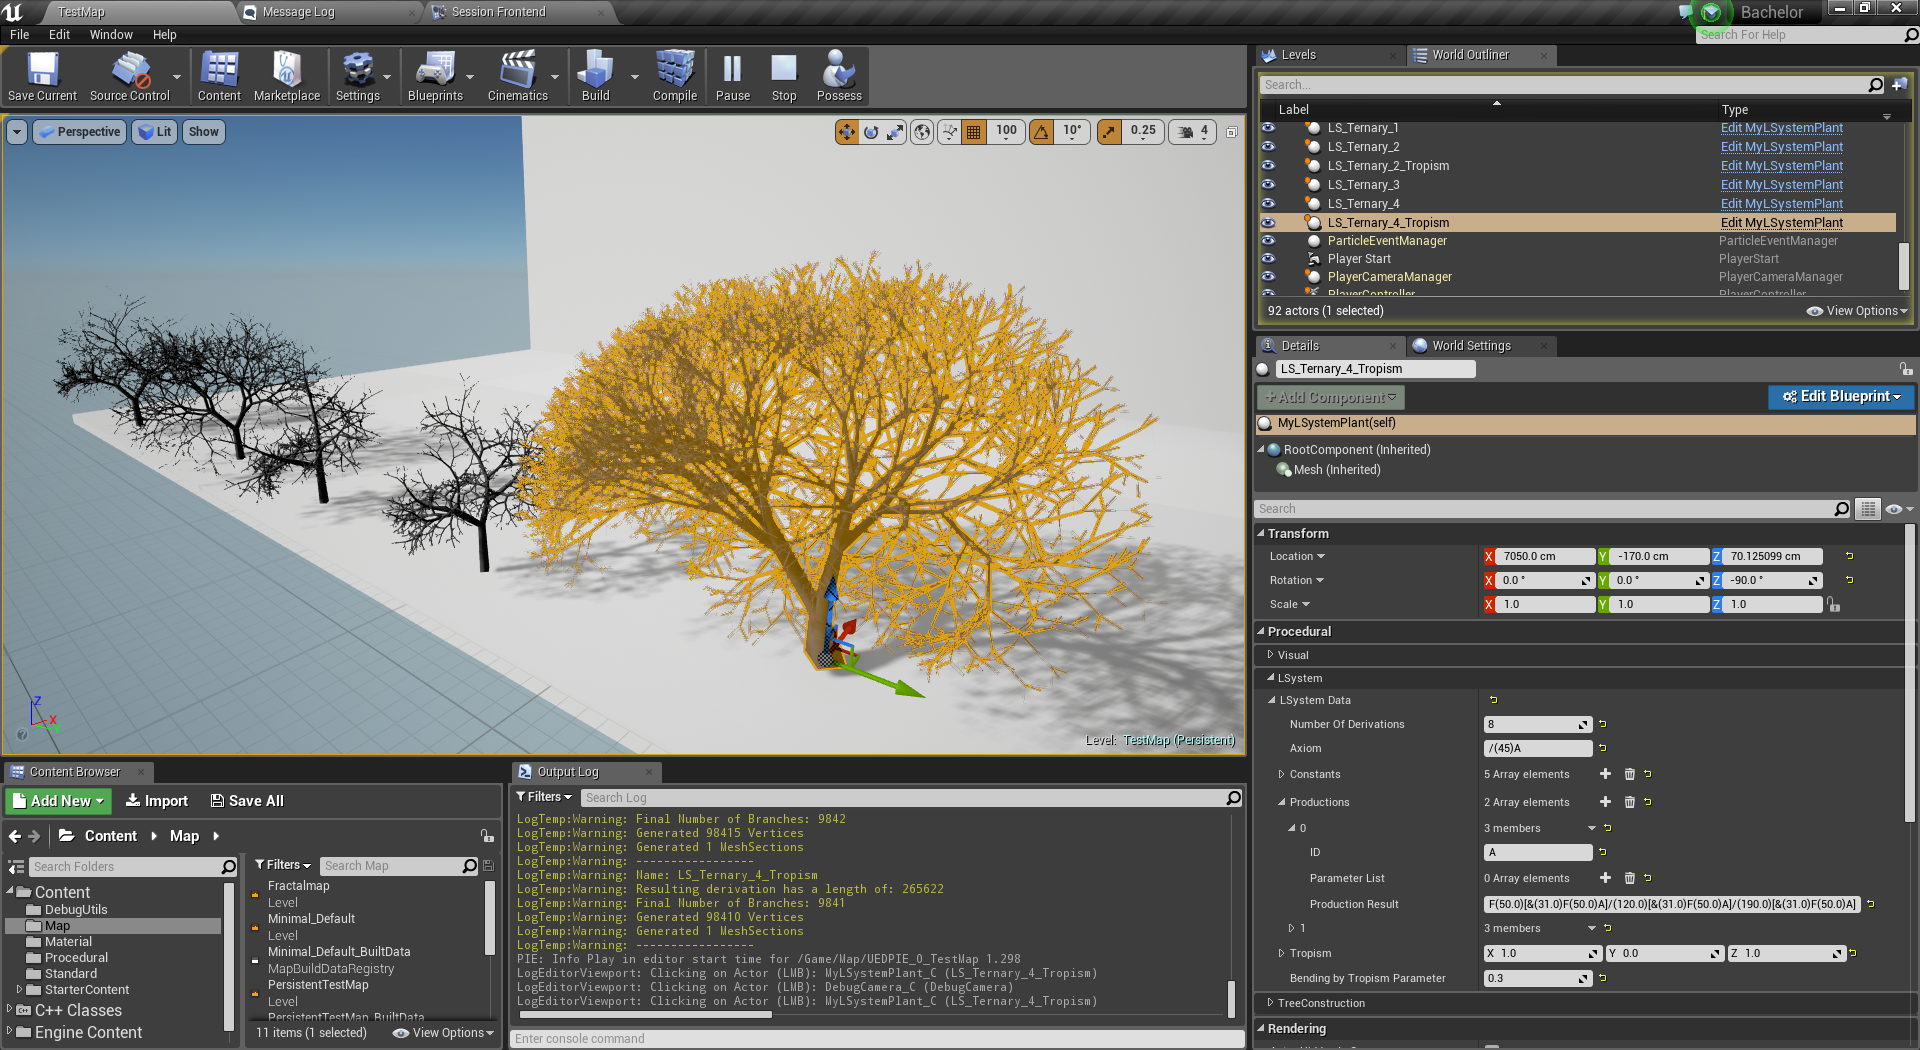
\includegraphics[width=\textwidth]{images/ScreenshotUE4Editor.png}
	\caption{Screenshot des visuellen Leveleditors der Unreal Engine 4. Der aktuell ausgewählte Actor und seine Komponenten sind gelb hervorgehoben. Die in der Bildmitte dargestellten Pfeile sowie die Eingabefelder im unteren rechten Bildbereich erlauben die Transformation des Actors. Ebenfalls im unteren rechten Bildbereich aufgelistet sind weitere Felder um die schnelle Änderung von Parameterwerten zu erlauben, die im $C++$ Quellcode entsprechend definiert sind. }
	\label{fig:ScreenshotUE4Editor}
\end{figure}


Die in den folgenden Kapiteln verwendete Längeneinheit entspricht der in Unreal Engine 4 verwendeten Einheit \grqq$cm$\grqq, das Winkelmaß entspricht der Einheit \glqq Grad\grqq. Alle Abbildungen von Baumstrukturen wurden mithilfe von Screenshots des, im Rahmen dieser Arbeit entwickelten, Projekts erstellt.

Der Aufbau des Projekts und der Zugriff auf die entwickelten Inhalte wird in Appendix \ref{ch:Projektaufbau} erläutert.